% Copyright © 2012-2014 Martin Ueding <dev@martin-ueding.de>

% This is my general purpose LaTeX header file for writing German documents.
% Ideally, you include this using a simple ``% Copyright © 2012-2014 Martin Ueding <dev@martin-ueding.de>

% This is my general purpose LaTeX header file for writing German documents.
% Ideally, you include this using a simple ``% Copyright © 2012-2014 Martin Ueding <dev@martin-ueding.de>

% This is my general purpose LaTeX header file for writing German documents.
% Ideally, you include this using a simple ``\input{header.tex}`` in your main
% document and start with ``\title`` and ``\begin{document}`` afterwards.

% If you need to add additional packages, I recommend not doing this in this
% file, but in your main document. That way, you can just drop in a new
% ``header.tex`` and get all the new commands without having to merge manually.

% Since this file encorporates a CC-BY-SA fragment, this whole files is
% licensed under the CC-BY-SA license.

\documentclass[11pt, ngerman, fleqn, DIV=15, headinclude, BCOR=2cm]{scrreprt}

\usepackage{graphicx}

\setkomafont{caption}{\sffamily}
\setkomafont{captionlabel}{\usekomafont{caption}}

%%%%%%%%%%%%%%%%%%%%%%%%%%%%%%%%%%%%%%%%%%%%%%%%%%%%%%%%%%%%%%%%%%%%%%%%%%%%%%%
%                                Locale, date                                 %
%%%%%%%%%%%%%%%%%%%%%%%%%%%%%%%%%%%%%%%%%%%%%%%%%%%%%%%%%%%%%%%%%%%%%%%%%%%%%%%

\usepackage{babel}
\usepackage[iso]{isodate}

%%%%%%%%%%%%%%%%%%%%%%%%%%%%%%%%%%%%%%%%%%%%%%%%%%%%%%%%%%%%%%%%%%%%%%%%%%%%%%%
%                          Margins and other spacing                          %
%%%%%%%%%%%%%%%%%%%%%%%%%%%%%%%%%%%%%%%%%%%%%%%%%%%%%%%%%%%%%%%%%%%%%%%%%%%%%%%

\usepackage[parfill]{parskip}
\usepackage{setspace}
\usepackage[activate]{microtype}

\setlength{\columnsep}{2cm}

%%%%%%%%%%%%%%%%%%%%%%%%%%%%%%%%%%%%%%%%%%%%%%%%%%%%%%%%%%%%%%%%%%%%%%%%%%%%%%%
%                                    Color                                    %
%%%%%%%%%%%%%%%%%%%%%%%%%%%%%%%%%%%%%%%%%%%%%%%%%%%%%%%%%%%%%%%%%%%%%%%%%%%%%%%

\usepackage[usenames, dvipsnames]{xcolor}

\colorlet{darkred}{red!70!black}
\colorlet{darkblue}{blue!70!black}
\colorlet{darkgreen}{green!40!black}

%%%%%%%%%%%%%%%%%%%%%%%%%%%%%%%%%%%%%%%%%%%%%%%%%%%%%%%%%%%%%%%%%%%%%%%%%%%%%%%
%                         Font and font like settings                         %
%%%%%%%%%%%%%%%%%%%%%%%%%%%%%%%%%%%%%%%%%%%%%%%%%%%%%%%%%%%%%%%%%%%%%%%%%%%%%%%

% This replaces all fonts with Bitstream Charter, Bitstream Vera Sans and
% Bitstream Vera Mono. Math will be rendered in Charter.
\usepackage[charter, greekuppercase=italicized]{mathdesign}
\usepackage{beramono}
\usepackage{berasans}

% Bold, sans-serif tensors. This fragment is taken from “egreg” from
% http://tex.stackexchange.com/a/82747/8945 and licensed under `CC-BY-SA
% <https://creativecommons.org/licenses/by-sa/3.0/>`_.
\usepackage{bm}
\DeclareMathAlphabet{\mathsfit}{\encodingdefault}{\sfdefault}{m}{sl}
\SetMathAlphabet{\mathsfit}{bold}{\encodingdefault}{\sfdefault}{bx}{sl}
\newcommand{\tens}[1]{\bm{\mathsfit{#1}}}

% Bold vectors.
\renewcommand{\vec}[1]{\boldsymbol{#1}}

%%%%%%%%%%%%%%%%%%%%%%%%%%%%%%%%%%%%%%%%%%%%%%%%%%%%%%%%%%%%%%%%%%%%%%%%%%%%%%%
%                               Input encoding                                %
%%%%%%%%%%%%%%%%%%%%%%%%%%%%%%%%%%%%%%%%%%%%%%%%%%%%%%%%%%%%%%%%%%%%%%%%%%%%%%%

\usepackage[T1]{fontenc}
\usepackage[utf8]{inputenc}

%%%%%%%%%%%%%%%%%%%%%%%%%%%%%%%%%%%%%%%%%%%%%%%%%%%%%%%%%%%%%%%%%%%%%%%%%%%%%%%
%                         Hyperrefs and PDF metadata                          %
%%%%%%%%%%%%%%%%%%%%%%%%%%%%%%%%%%%%%%%%%%%%%%%%%%%%%%%%%%%%%%%%%%%%%%%%%%%%%%%

\usepackage{hyperref}

% This sets the author in the properties of the PDF as well. If you want to
% change it, just override it with another ``\hypersetup`` call.
\hypersetup{
    breaklinks=false,
    citecolor=darkgreen,
    colorlinks=true,
    linkcolor=darkblue,
    menucolor=black,
    pdfauthor={Martin Ueding},
    urlcolor=darkblue,
}

%%%%%%%%%%%%%%%%%%%%%%%%%%%%%%%%%%%%%%%%%%%%%%%%%%%%%%%%%%%%%%%%%%%%%%%%%%%%%%%
%                               Math Operators                                %
%%%%%%%%%%%%%%%%%%%%%%%%%%%%%%%%%%%%%%%%%%%%%%%%%%%%%%%%%%%%%%%%%%%%%%%%%%%%%%%

% AMS environments like ``align`` and theorems like ``proof``.
\usepackage{amsmath}
\usepackage{amsthm}

% Common math constructs like partial derivatives.
\usepackage{commath}

% Physical units.
\usepackage[output-decimal-marker={,}]{siunitx}

% Since I use mathdesign with italic uppercase greek characters, the Ohm unit will be displayed with an italic Ω by default. Units have to be roman, so this forces it the right way.
\DeclareSIUnit{\ohm}{$\Omegaup$}
\DeclareSIUnit{\division}{DIV}
\DeclareSIUnit{\voltss}{$\mathrm{V_{SS}}$}

% Word like operators.
\DeclareMathOperator{\acosh}{arcosh}
\DeclareMathOperator{\arcosh}{arcosh}
\DeclareMathOperator{\arcsinh}{arsinh}
\DeclareMathOperator{\arsinh}{arsinh}
\DeclareMathOperator{\asinh}{arsinh}
\DeclareMathOperator{\card}{card}
\DeclareMathOperator{\csch}{csch}
\DeclareMathOperator{\diam}{diam}
\DeclareMathOperator{\sech}{sech}
\renewcommand{\Im}{\mathop{{}\mathrm{Im}}\nolimits}
\renewcommand{\Re}{\mathop{{}\mathrm{Re}}\nolimits}

% Fourier transform.
\DeclareMathOperator{\fourier}{\ensuremath{\mathcal{F}}}

% Roman versions of “e” and “i” to serve as Euler's number and the imaginary
% constant.
\newcommand{\eup}{\mathrm e}
\newcommand{\iup}{\mathrm i}

% Symbols for the various mathematical fields (natural numbers, integers,
% rational numbers, real numbers, complex numbers).
\newcommand{\C}{\ensuremath{\mathbb C}}
\newcommand{\N}{\ensuremath{\mathbb N}}
\newcommand{\Q}{\ensuremath{\mathbb Q}}
\newcommand{\R}{\ensuremath{\mathbb R}}
\newcommand{\Z}{\ensuremath{\mathbb Z}}

% Shape like operators.
\DeclareMathOperator{\dalambert}{\Box}
\DeclareMathOperator{\laplace}{\bigtriangleup}
\newcommand{\curl}{\vnabla \times}
\newcommand{\divergence}[1]{\inner{\vnabla}{#1}}
\newcommand{\Divergence}[1]{\Inner{\vnabla}{#1}}
\newcommand{\vnabla}{\vec \nabla}

\newcommand{\half}{\frac 12}

% Unit vector (German „Einheitsvektor“).
\newcommand{\ev}{\hat{\vec e}}

% Mathematician's notation for the inner (scalar, dot) product.
\newcommand{\bracket}[1]{\langle #1 \rangle}
\newcommand{\Bracket}[1]{\left\langle #1 \right\rangle}
\newcommand{\inner}[2]{\bracket{#1, #2}}
\newcommand{\Inner}[2]{\Bracket{#1, #2}}

% Placeholders.
\newcommand{\fehlt}{\textcolor{darkred}{Hier fehlen noch Inhalte.}}
\newcommand{\messwert}{\textcolor{blue}{\square}}
\newcommand{\punkte}{\phantom{xxxxx}}

% Separator for equations on a single line.
\newcommand{\eqnsep}{,\quad}

% Quantum Mechanics.
\usepackage{braket}

% Thermodynamic partial derivative.
\newcommand\tdpd[3]{\del{\dpd{#1}{#2}}_{#3}}

%%%%%%%%%%%%%%%%%%%%%%%%%%%%%%%%%%%%%%%%%%%%%%%%%%%%%%%%%%%%%%%%%%%%%%%%%%%%%%%
%                                  Headings                                   %
%%%%%%%%%%%%%%%%%%%%%%%%%%%%%%%%%%%%%%%%%%%%%%%%%%%%%%%%%%%%%%%%%%%%%%%%%%%%%%%

% This will set fancy headings to the top of the page. The page number will be
% accompanied by the total number of pages. That way, you will know if any page
% is missing.
%
% If you do not want this for your document, you can just use
% ``\pagestyle{plain}``.

\usepackage{scrpage2}

\pagestyle{scrheadings}
\automark{section}
\chead{}
\ihead{}
\ohead{\rightmark}
\setheadsepline{.4pt}

%%%%%%%%%%%%%%%%%%%%%%%%%%%%%%%%%%%%%%%%%%%%%%%%%%%%%%%%%%%%%%%%%%%%%%%%%%%%%%%
%                            Bibliography (BibTeX)                            %
%%%%%%%%%%%%%%%%%%%%%%%%%%%%%%%%%%%%%%%%%%%%%%%%%%%%%%%%%%%%%%%%%%%%%%%%%%%%%%%

\newcommand{\bibliographyfile}{../../central-bibtex/Central}

\usepackage[
    backend=bibtex,
    style=alphabetic,
    %isbn=false,
    %pagetracker=false,
    %maxbibnames=50,
    %maxcitenames=2,
    %autocite=inline,
    %block=space,
    %backref=false,
    %backrefstyle=three+,
    %date=short,
    hyperref=true
]{biblatex}

\setlength{\bibitemsep}{.7em}
\setlength{\bibhang}{4ex}

\IfFileExists{\bibliographyfile}{
    \bibliography{\bibliographyfile}
}{}

%%%%%%%%%%%%%%%%%%%%%%%%%%%%%%%%%%%%%%%%%%%%%%%%%%%%%%%%%%%%%%%%%%%%%%%%%%%%%%%
%                                Abbreviations                                %
%%%%%%%%%%%%%%%%%%%%%%%%%%%%%%%%%%%%%%%%%%%%%%%%%%%%%%%%%%%%%%%%%%%%%%%%%%%%%%%

\newcommand{\dhabk}{\mbox{d.\,h.}}

%%%%%%%%%%%%%%%%%%%%%%%%%%%%%%%%%%%%%%%%%%%%%%%%%%%%%%%%%%%%%%%%%%%%%%%%%%%%%%%
%                                  Licences                                   %
%%%%%%%%%%%%%%%%%%%%%%%%%%%%%%%%%%%%%%%%%%%%%%%%%%%%%%%%%%%%%%%%%%%%%%%%%%%%%%%

\usepackage{ccicons}

\newcommand{\ccbysadetext}{%
    \begin{small}
        Dieses Werk bzw. Inhalt steht unter einer
        \href{http://creativecommons.org/licenses/by-sa/3.0/deed.de}{%
            Creative Commons Namensnennung - Weitergabe unter gleichen
        Bedingungen 3.0 Unported Lizenz}.
    \end{small}
}

\newcommand{\ccbysadetitle}{%
    Lizenz: \href{http://creativecommons.org/licenses/by-sa/3.0/deed.de}
    {CC-BY-SA 3.0 \ccbysa}
}

\newcommand\erklaerungFehlerNotation{%
    In dieser Notation bedeutet \num{1.234 +- 0.005}, dass der Wert
    $\num{1.234} \pm \num{0.005}$ ist. Die Ziffern in Klammern sind die
    Fehlerangabe. Um den Fehler zu erhalten, wird diese von rechts über die
    Zahl gelegt, alle anderen Stellen werden auf 0 gesetzt.
}

`` in your main
% document and start with ``\title`` and ``\begin{document}`` afterwards.

% If you need to add additional packages, I recommend not doing this in this
% file, but in your main document. That way, you can just drop in a new
% ``header.tex`` and get all the new commands without having to merge manually.

% Since this file encorporates a CC-BY-SA fragment, this whole files is
% licensed under the CC-BY-SA license.

\documentclass[11pt, ngerman, fleqn, DIV=15, headinclude, BCOR=2cm]{scrreprt}

\usepackage{graphicx}

\setkomafont{caption}{\sffamily}
\setkomafont{captionlabel}{\usekomafont{caption}}

%%%%%%%%%%%%%%%%%%%%%%%%%%%%%%%%%%%%%%%%%%%%%%%%%%%%%%%%%%%%%%%%%%%%%%%%%%%%%%%
%                                Locale, date                                 %
%%%%%%%%%%%%%%%%%%%%%%%%%%%%%%%%%%%%%%%%%%%%%%%%%%%%%%%%%%%%%%%%%%%%%%%%%%%%%%%

\usepackage{babel}
\usepackage[iso]{isodate}

%%%%%%%%%%%%%%%%%%%%%%%%%%%%%%%%%%%%%%%%%%%%%%%%%%%%%%%%%%%%%%%%%%%%%%%%%%%%%%%
%                          Margins and other spacing                          %
%%%%%%%%%%%%%%%%%%%%%%%%%%%%%%%%%%%%%%%%%%%%%%%%%%%%%%%%%%%%%%%%%%%%%%%%%%%%%%%

\usepackage[parfill]{parskip}
\usepackage{setspace}
\usepackage[activate]{microtype}

\setlength{\columnsep}{2cm}

%%%%%%%%%%%%%%%%%%%%%%%%%%%%%%%%%%%%%%%%%%%%%%%%%%%%%%%%%%%%%%%%%%%%%%%%%%%%%%%
%                                    Color                                    %
%%%%%%%%%%%%%%%%%%%%%%%%%%%%%%%%%%%%%%%%%%%%%%%%%%%%%%%%%%%%%%%%%%%%%%%%%%%%%%%

\usepackage[usenames, dvipsnames]{xcolor}

\colorlet{darkred}{red!70!black}
\colorlet{darkblue}{blue!70!black}
\colorlet{darkgreen}{green!40!black}

%%%%%%%%%%%%%%%%%%%%%%%%%%%%%%%%%%%%%%%%%%%%%%%%%%%%%%%%%%%%%%%%%%%%%%%%%%%%%%%
%                         Font and font like settings                         %
%%%%%%%%%%%%%%%%%%%%%%%%%%%%%%%%%%%%%%%%%%%%%%%%%%%%%%%%%%%%%%%%%%%%%%%%%%%%%%%

% This replaces all fonts with Bitstream Charter, Bitstream Vera Sans and
% Bitstream Vera Mono. Math will be rendered in Charter.
\usepackage[charter, greekuppercase=italicized]{mathdesign}
\usepackage{beramono}
\usepackage{berasans}

% Bold, sans-serif tensors. This fragment is taken from “egreg” from
% http://tex.stackexchange.com/a/82747/8945 and licensed under `CC-BY-SA
% <https://creativecommons.org/licenses/by-sa/3.0/>`_.
\usepackage{bm}
\DeclareMathAlphabet{\mathsfit}{\encodingdefault}{\sfdefault}{m}{sl}
\SetMathAlphabet{\mathsfit}{bold}{\encodingdefault}{\sfdefault}{bx}{sl}
\newcommand{\tens}[1]{\bm{\mathsfit{#1}}}

% Bold vectors.
\renewcommand{\vec}[1]{\boldsymbol{#1}}

%%%%%%%%%%%%%%%%%%%%%%%%%%%%%%%%%%%%%%%%%%%%%%%%%%%%%%%%%%%%%%%%%%%%%%%%%%%%%%%
%                               Input encoding                                %
%%%%%%%%%%%%%%%%%%%%%%%%%%%%%%%%%%%%%%%%%%%%%%%%%%%%%%%%%%%%%%%%%%%%%%%%%%%%%%%

\usepackage[T1]{fontenc}
\usepackage[utf8]{inputenc}

%%%%%%%%%%%%%%%%%%%%%%%%%%%%%%%%%%%%%%%%%%%%%%%%%%%%%%%%%%%%%%%%%%%%%%%%%%%%%%%
%                         Hyperrefs and PDF metadata                          %
%%%%%%%%%%%%%%%%%%%%%%%%%%%%%%%%%%%%%%%%%%%%%%%%%%%%%%%%%%%%%%%%%%%%%%%%%%%%%%%

\usepackage{hyperref}

% This sets the author in the properties of the PDF as well. If you want to
% change it, just override it with another ``\hypersetup`` call.
\hypersetup{
    breaklinks=false,
    citecolor=darkgreen,
    colorlinks=true,
    linkcolor=darkblue,
    menucolor=black,
    pdfauthor={Martin Ueding},
    urlcolor=darkblue,
}

%%%%%%%%%%%%%%%%%%%%%%%%%%%%%%%%%%%%%%%%%%%%%%%%%%%%%%%%%%%%%%%%%%%%%%%%%%%%%%%
%                               Math Operators                                %
%%%%%%%%%%%%%%%%%%%%%%%%%%%%%%%%%%%%%%%%%%%%%%%%%%%%%%%%%%%%%%%%%%%%%%%%%%%%%%%

% AMS environments like ``align`` and theorems like ``proof``.
\usepackage{amsmath}
\usepackage{amsthm}

% Common math constructs like partial derivatives.
\usepackage{commath}

% Physical units.
\usepackage[output-decimal-marker={,}]{siunitx}

% Since I use mathdesign with italic uppercase greek characters, the Ohm unit will be displayed with an italic Ω by default. Units have to be roman, so this forces it the right way.
\DeclareSIUnit{\ohm}{$\Omegaup$}
\DeclareSIUnit{\division}{DIV}
\DeclareSIUnit{\voltss}{$\mathrm{V_{SS}}$}

% Word like operators.
\DeclareMathOperator{\acosh}{arcosh}
\DeclareMathOperator{\arcosh}{arcosh}
\DeclareMathOperator{\arcsinh}{arsinh}
\DeclareMathOperator{\arsinh}{arsinh}
\DeclareMathOperator{\asinh}{arsinh}
\DeclareMathOperator{\card}{card}
\DeclareMathOperator{\csch}{csch}
\DeclareMathOperator{\diam}{diam}
\DeclareMathOperator{\sech}{sech}
\renewcommand{\Im}{\mathop{{}\mathrm{Im}}\nolimits}
\renewcommand{\Re}{\mathop{{}\mathrm{Re}}\nolimits}

% Fourier transform.
\DeclareMathOperator{\fourier}{\ensuremath{\mathcal{F}}}

% Roman versions of “e” and “i” to serve as Euler's number and the imaginary
% constant.
\newcommand{\eup}{\mathrm e}
\newcommand{\iup}{\mathrm i}

% Symbols for the various mathematical fields (natural numbers, integers,
% rational numbers, real numbers, complex numbers).
\newcommand{\C}{\ensuremath{\mathbb C}}
\newcommand{\N}{\ensuremath{\mathbb N}}
\newcommand{\Q}{\ensuremath{\mathbb Q}}
\newcommand{\R}{\ensuremath{\mathbb R}}
\newcommand{\Z}{\ensuremath{\mathbb Z}}

% Shape like operators.
\DeclareMathOperator{\dalambert}{\Box}
\DeclareMathOperator{\laplace}{\bigtriangleup}
\newcommand{\curl}{\vnabla \times}
\newcommand{\divergence}[1]{\inner{\vnabla}{#1}}
\newcommand{\Divergence}[1]{\Inner{\vnabla}{#1}}
\newcommand{\vnabla}{\vec \nabla}

\newcommand{\half}{\frac 12}

% Unit vector (German „Einheitsvektor“).
\newcommand{\ev}{\hat{\vec e}}

% Mathematician's notation for the inner (scalar, dot) product.
\newcommand{\bracket}[1]{\langle #1 \rangle}
\newcommand{\Bracket}[1]{\left\langle #1 \right\rangle}
\newcommand{\inner}[2]{\bracket{#1, #2}}
\newcommand{\Inner}[2]{\Bracket{#1, #2}}

% Placeholders.
\newcommand{\fehlt}{\textcolor{darkred}{Hier fehlen noch Inhalte.}}
\newcommand{\messwert}{\textcolor{blue}{\square}}
\newcommand{\punkte}{\phantom{xxxxx}}

% Separator for equations on a single line.
\newcommand{\eqnsep}{,\quad}

% Quantum Mechanics.
\usepackage{braket}

% Thermodynamic partial derivative.
\newcommand\tdpd[3]{\del{\dpd{#1}{#2}}_{#3}}

%%%%%%%%%%%%%%%%%%%%%%%%%%%%%%%%%%%%%%%%%%%%%%%%%%%%%%%%%%%%%%%%%%%%%%%%%%%%%%%
%                                  Headings                                   %
%%%%%%%%%%%%%%%%%%%%%%%%%%%%%%%%%%%%%%%%%%%%%%%%%%%%%%%%%%%%%%%%%%%%%%%%%%%%%%%

% This will set fancy headings to the top of the page. The page number will be
% accompanied by the total number of pages. That way, you will know if any page
% is missing.
%
% If you do not want this for your document, you can just use
% ``\pagestyle{plain}``.

\usepackage{scrpage2}

\pagestyle{scrheadings}
\automark{section}
\chead{}
\ihead{}
\ohead{\rightmark}
\setheadsepline{.4pt}

%%%%%%%%%%%%%%%%%%%%%%%%%%%%%%%%%%%%%%%%%%%%%%%%%%%%%%%%%%%%%%%%%%%%%%%%%%%%%%%
%                            Bibliography (BibTeX)                            %
%%%%%%%%%%%%%%%%%%%%%%%%%%%%%%%%%%%%%%%%%%%%%%%%%%%%%%%%%%%%%%%%%%%%%%%%%%%%%%%

\newcommand{\bibliographyfile}{../../central-bibtex/Central}

\usepackage[
    backend=bibtex,
    style=alphabetic,
    %isbn=false,
    %pagetracker=false,
    %maxbibnames=50,
    %maxcitenames=2,
    %autocite=inline,
    %block=space,
    %backref=false,
    %backrefstyle=three+,
    %date=short,
    hyperref=true
]{biblatex}

\setlength{\bibitemsep}{.7em}
\setlength{\bibhang}{4ex}

\IfFileExists{\bibliographyfile}{
    \bibliography{\bibliographyfile}
}{}

%%%%%%%%%%%%%%%%%%%%%%%%%%%%%%%%%%%%%%%%%%%%%%%%%%%%%%%%%%%%%%%%%%%%%%%%%%%%%%%
%                                Abbreviations                                %
%%%%%%%%%%%%%%%%%%%%%%%%%%%%%%%%%%%%%%%%%%%%%%%%%%%%%%%%%%%%%%%%%%%%%%%%%%%%%%%

\newcommand{\dhabk}{\mbox{d.\,h.}}

%%%%%%%%%%%%%%%%%%%%%%%%%%%%%%%%%%%%%%%%%%%%%%%%%%%%%%%%%%%%%%%%%%%%%%%%%%%%%%%
%                                  Licences                                   %
%%%%%%%%%%%%%%%%%%%%%%%%%%%%%%%%%%%%%%%%%%%%%%%%%%%%%%%%%%%%%%%%%%%%%%%%%%%%%%%

\usepackage{ccicons}

\newcommand{\ccbysadetext}{%
    \begin{small}
        Dieses Werk bzw. Inhalt steht unter einer
        \href{http://creativecommons.org/licenses/by-sa/3.0/deed.de}{%
            Creative Commons Namensnennung - Weitergabe unter gleichen
        Bedingungen 3.0 Unported Lizenz}.
    \end{small}
}

\newcommand{\ccbysadetitle}{%
    Lizenz: \href{http://creativecommons.org/licenses/by-sa/3.0/deed.de}
    {CC-BY-SA 3.0 \ccbysa}
}

\newcommand\erklaerungFehlerNotation{%
    In dieser Notation bedeutet \num{1.234 +- 0.005}, dass der Wert
    $\num{1.234} \pm \num{0.005}$ ist. Die Ziffern in Klammern sind die
    Fehlerangabe. Um den Fehler zu erhalten, wird diese von rechts über die
    Zahl gelegt, alle anderen Stellen werden auf 0 gesetzt.
}

`` in your main
% document and start with ``\title`` and ``\begin{document}`` afterwards.

% If you need to add additional packages, I recommend not doing this in this
% file, but in your main document. That way, you can just drop in a new
% ``header.tex`` and get all the new commands without having to merge manually.

% Since this file encorporates a CC-BY-SA fragment, this whole files is
% licensed under the CC-BY-SA license.

\documentclass[11pt, ngerman, fleqn, DIV=15, headinclude, BCOR=2cm]{scrreprt}

\usepackage{graphicx}

\setkomafont{caption}{\sffamily}
\setkomafont{captionlabel}{\usekomafont{caption}}

%%%%%%%%%%%%%%%%%%%%%%%%%%%%%%%%%%%%%%%%%%%%%%%%%%%%%%%%%%%%%%%%%%%%%%%%%%%%%%%
%                                Locale, date                                 %
%%%%%%%%%%%%%%%%%%%%%%%%%%%%%%%%%%%%%%%%%%%%%%%%%%%%%%%%%%%%%%%%%%%%%%%%%%%%%%%

\usepackage{babel}
\usepackage[iso]{isodate}

%%%%%%%%%%%%%%%%%%%%%%%%%%%%%%%%%%%%%%%%%%%%%%%%%%%%%%%%%%%%%%%%%%%%%%%%%%%%%%%
%                          Margins and other spacing                          %
%%%%%%%%%%%%%%%%%%%%%%%%%%%%%%%%%%%%%%%%%%%%%%%%%%%%%%%%%%%%%%%%%%%%%%%%%%%%%%%

\usepackage[parfill]{parskip}
\usepackage{setspace}
\usepackage[activate]{microtype}

\setlength{\columnsep}{2cm}

%%%%%%%%%%%%%%%%%%%%%%%%%%%%%%%%%%%%%%%%%%%%%%%%%%%%%%%%%%%%%%%%%%%%%%%%%%%%%%%
%                                    Color                                    %
%%%%%%%%%%%%%%%%%%%%%%%%%%%%%%%%%%%%%%%%%%%%%%%%%%%%%%%%%%%%%%%%%%%%%%%%%%%%%%%

\usepackage[usenames, dvipsnames]{xcolor}

\colorlet{darkred}{red!70!black}
\colorlet{darkblue}{blue!70!black}
\colorlet{darkgreen}{green!40!black}

%%%%%%%%%%%%%%%%%%%%%%%%%%%%%%%%%%%%%%%%%%%%%%%%%%%%%%%%%%%%%%%%%%%%%%%%%%%%%%%
%                         Font and font like settings                         %
%%%%%%%%%%%%%%%%%%%%%%%%%%%%%%%%%%%%%%%%%%%%%%%%%%%%%%%%%%%%%%%%%%%%%%%%%%%%%%%

% This replaces all fonts with Bitstream Charter, Bitstream Vera Sans and
% Bitstream Vera Mono. Math will be rendered in Charter.
\usepackage[charter, greekuppercase=italicized]{mathdesign}
\usepackage{beramono}
\usepackage{berasans}

% Bold, sans-serif tensors. This fragment is taken from “egreg” from
% http://tex.stackexchange.com/a/82747/8945 and licensed under `CC-BY-SA
% <https://creativecommons.org/licenses/by-sa/3.0/>`_.
\usepackage{bm}
\DeclareMathAlphabet{\mathsfit}{\encodingdefault}{\sfdefault}{m}{sl}
\SetMathAlphabet{\mathsfit}{bold}{\encodingdefault}{\sfdefault}{bx}{sl}
\newcommand{\tens}[1]{\bm{\mathsfit{#1}}}

% Bold vectors.
\renewcommand{\vec}[1]{\boldsymbol{#1}}

%%%%%%%%%%%%%%%%%%%%%%%%%%%%%%%%%%%%%%%%%%%%%%%%%%%%%%%%%%%%%%%%%%%%%%%%%%%%%%%
%                               Input encoding                                %
%%%%%%%%%%%%%%%%%%%%%%%%%%%%%%%%%%%%%%%%%%%%%%%%%%%%%%%%%%%%%%%%%%%%%%%%%%%%%%%

\usepackage[T1]{fontenc}
\usepackage[utf8]{inputenc}

%%%%%%%%%%%%%%%%%%%%%%%%%%%%%%%%%%%%%%%%%%%%%%%%%%%%%%%%%%%%%%%%%%%%%%%%%%%%%%%
%                         Hyperrefs and PDF metadata                          %
%%%%%%%%%%%%%%%%%%%%%%%%%%%%%%%%%%%%%%%%%%%%%%%%%%%%%%%%%%%%%%%%%%%%%%%%%%%%%%%

\usepackage{hyperref}

% This sets the author in the properties of the PDF as well. If you want to
% change it, just override it with another ``\hypersetup`` call.
\hypersetup{
    breaklinks=false,
    citecolor=darkgreen,
    colorlinks=true,
    linkcolor=darkblue,
    menucolor=black,
    pdfauthor={Martin Ueding},
    urlcolor=darkblue,
}

%%%%%%%%%%%%%%%%%%%%%%%%%%%%%%%%%%%%%%%%%%%%%%%%%%%%%%%%%%%%%%%%%%%%%%%%%%%%%%%
%                               Math Operators                                %
%%%%%%%%%%%%%%%%%%%%%%%%%%%%%%%%%%%%%%%%%%%%%%%%%%%%%%%%%%%%%%%%%%%%%%%%%%%%%%%

% AMS environments like ``align`` and theorems like ``proof``.
\usepackage{amsmath}
\usepackage{amsthm}

% Common math constructs like partial derivatives.
\usepackage{commath}

% Physical units.
\usepackage[output-decimal-marker={,}]{siunitx}

% Since I use mathdesign with italic uppercase greek characters, the Ohm unit will be displayed with an italic Ω by default. Units have to be roman, so this forces it the right way.
\DeclareSIUnit{\ohm}{$\Omegaup$}
\DeclareSIUnit{\division}{DIV}
\DeclareSIUnit{\voltss}{$\mathrm{V_{SS}}$}

% Word like operators.
\DeclareMathOperator{\acosh}{arcosh}
\DeclareMathOperator{\arcosh}{arcosh}
\DeclareMathOperator{\arcsinh}{arsinh}
\DeclareMathOperator{\arsinh}{arsinh}
\DeclareMathOperator{\asinh}{arsinh}
\DeclareMathOperator{\card}{card}
\DeclareMathOperator{\csch}{csch}
\DeclareMathOperator{\diam}{diam}
\DeclareMathOperator{\sech}{sech}
\renewcommand{\Im}{\mathop{{}\mathrm{Im}}\nolimits}
\renewcommand{\Re}{\mathop{{}\mathrm{Re}}\nolimits}

% Fourier transform.
\DeclareMathOperator{\fourier}{\ensuremath{\mathcal{F}}}

% Roman versions of “e” and “i” to serve as Euler's number and the imaginary
% constant.
\newcommand{\eup}{\mathrm e}
\newcommand{\iup}{\mathrm i}

% Symbols for the various mathematical fields (natural numbers, integers,
% rational numbers, real numbers, complex numbers).
\newcommand{\C}{\ensuremath{\mathbb C}}
\newcommand{\N}{\ensuremath{\mathbb N}}
\newcommand{\Q}{\ensuremath{\mathbb Q}}
\newcommand{\R}{\ensuremath{\mathbb R}}
\newcommand{\Z}{\ensuremath{\mathbb Z}}

% Shape like operators.
\DeclareMathOperator{\dalambert}{\Box}
\DeclareMathOperator{\laplace}{\bigtriangleup}
\newcommand{\curl}{\vnabla \times}
\newcommand{\divergence}[1]{\inner{\vnabla}{#1}}
\newcommand{\Divergence}[1]{\Inner{\vnabla}{#1}}
\newcommand{\vnabla}{\vec \nabla}

\newcommand{\half}{\frac 12}

% Unit vector (German „Einheitsvektor“).
\newcommand{\ev}{\hat{\vec e}}

% Mathematician's notation for the inner (scalar, dot) product.
\newcommand{\bracket}[1]{\langle #1 \rangle}
\newcommand{\Bracket}[1]{\left\langle #1 \right\rangle}
\newcommand{\inner}[2]{\bracket{#1, #2}}
\newcommand{\Inner}[2]{\Bracket{#1, #2}}

% Placeholders.
\newcommand{\fehlt}{\textcolor{darkred}{Hier fehlen noch Inhalte.}}
\newcommand{\messwert}{\textcolor{blue}{\square}}
\newcommand{\punkte}{\phantom{xxxxx}}

% Separator for equations on a single line.
\newcommand{\eqnsep}{,\quad}

% Quantum Mechanics.
\usepackage{braket}

% Thermodynamic partial derivative.
\newcommand\tdpd[3]{\del{\dpd{#1}{#2}}_{#3}}

%%%%%%%%%%%%%%%%%%%%%%%%%%%%%%%%%%%%%%%%%%%%%%%%%%%%%%%%%%%%%%%%%%%%%%%%%%%%%%%
%                                  Headings                                   %
%%%%%%%%%%%%%%%%%%%%%%%%%%%%%%%%%%%%%%%%%%%%%%%%%%%%%%%%%%%%%%%%%%%%%%%%%%%%%%%

% This will set fancy headings to the top of the page. The page number will be
% accompanied by the total number of pages. That way, you will know if any page
% is missing.
%
% If you do not want this for your document, you can just use
% ``\pagestyle{plain}``.

\usepackage{scrpage2}

\pagestyle{scrheadings}
\automark{section}
\chead{}
\ihead{}
\ohead{\rightmark}
\setheadsepline{.4pt}

%%%%%%%%%%%%%%%%%%%%%%%%%%%%%%%%%%%%%%%%%%%%%%%%%%%%%%%%%%%%%%%%%%%%%%%%%%%%%%%
%                            Bibliography (BibTeX)                            %
%%%%%%%%%%%%%%%%%%%%%%%%%%%%%%%%%%%%%%%%%%%%%%%%%%%%%%%%%%%%%%%%%%%%%%%%%%%%%%%

\newcommand{\bibliographyfile}{../../central-bibtex/Central}

\usepackage[
    backend=bibtex,
    style=alphabetic,
    %isbn=false,
    %pagetracker=false,
    %maxbibnames=50,
    %maxcitenames=2,
    %autocite=inline,
    %block=space,
    %backref=false,
    %backrefstyle=three+,
    %date=short,
    hyperref=true
]{biblatex}

\setlength{\bibitemsep}{.7em}
\setlength{\bibhang}{4ex}

\IfFileExists{\bibliographyfile}{
    \bibliography{\bibliographyfile}
}{}

%%%%%%%%%%%%%%%%%%%%%%%%%%%%%%%%%%%%%%%%%%%%%%%%%%%%%%%%%%%%%%%%%%%%%%%%%%%%%%%
%                                Abbreviations                                %
%%%%%%%%%%%%%%%%%%%%%%%%%%%%%%%%%%%%%%%%%%%%%%%%%%%%%%%%%%%%%%%%%%%%%%%%%%%%%%%

\newcommand{\dhabk}{\mbox{d.\,h.}}

%%%%%%%%%%%%%%%%%%%%%%%%%%%%%%%%%%%%%%%%%%%%%%%%%%%%%%%%%%%%%%%%%%%%%%%%%%%%%%%
%                                  Licences                                   %
%%%%%%%%%%%%%%%%%%%%%%%%%%%%%%%%%%%%%%%%%%%%%%%%%%%%%%%%%%%%%%%%%%%%%%%%%%%%%%%

\usepackage{ccicons}

\newcommand{\ccbysadetext}{%
    \begin{small}
        Dieses Werk bzw. Inhalt steht unter einer
        \href{http://creativecommons.org/licenses/by-sa/3.0/deed.de}{%
            Creative Commons Namensnennung - Weitergabe unter gleichen
        Bedingungen 3.0 Unported Lizenz}.
    \end{small}
}

\newcommand{\ccbysadetitle}{%
    Lizenz: \href{http://creativecommons.org/licenses/by-sa/3.0/deed.de}
    {CC-BY-SA 3.0 \ccbysa}
}

\newcommand\erklaerungFehlerNotation{%
    In dieser Notation bedeutet \num{1.234 +- 0.005}, dass der Wert
    $\num{1.234} \pm \num{0.005}$ ist. Die Ziffern in Klammern sind die
    Fehlerangabe. Um den Fehler zu erhalten, wird diese von rechts über die
    Zahl gelegt, alle anderen Stellen werden auf 0 gesetzt.
}



\usepackage[section]{placeins}

\usepackage{csquotes}

\usepackage{tikz}
\usetikzlibrary{chains}
\usetikzlibrary{shapes.geometric}

\tikzset{device/.style={
                rectangle,
                minimum size=6mm,
                draw=black
            },
            monitor/.style={
                rectangle,
                rounded corners=2mm,
                minimum size=6mm,
                draw=black
            },
        }

\usepackage{pgfplots}
\pgfplotsset{
    compat=1.5,
    width=0.8\linewidth,
    xticklabel style={/pgf/number format/use comma},
    yticklabel style={/pgf/number format/use comma},
}

\usepgfplotslibrary{external}
\tikzexternalize

\usepackage{booktabs}

\hypersetup{
    pdftitle=
}

\subject{Praktikumsprotokoll}
\title{$\boldsymbol\betaup$-Spektrometer}
\subtitle{Versuch P523 -- Universität Bonn}
\author{
    Martin Ueding \\ \small{\href{mailto:mu@martin-ueding.de}{mu@martin-ueding.de}}
    \and
    Lino Lemmer \\
    \small{\href{mailto:l2@uni-bonn.de}{l2@uni-bonn.de}}
}

\date{\daterange{2014-04-24}{2014-04-25}}

% TODO Tutor Eintragen
%\publishers{Tutor: TODO}

\begin{document}

\maketitle


\begin{abstract}
    In diesem Versuch kalibrieren wir ein doppeltfokussierendes $\piup
    \sqrt2$-Spektrometer mit $^{137}$Ba und bestimmen das Auflösungsvermögen.
    Wir nehmen die $\betaup$-Spektren von $^{22}$Na und $^{204}$Tl auf. Aus den
    Messdaten bestimmen wir die Maximalenergie der emittierten Teilchen.
\end{abstract}

\tableofcontents

\chapter{Theorie}

\section{Zerfallsarten}

\newcommand\betaplus{\betaup^+}
\newcommand\betaminus{\betaup^-}

Instabile Kerne können über verschiedene Kanäle zerfallen. Die für diesen
Versuch Interessanten sind die $\betaplus$- und $\betaminus$-Zerfälle sowie der
Elektroneneinfang.

Bei $\betaminus$-Zerfall passiert auf Quarkebene folgendes:
\[
    \mathrm d
    \quad\rightharpoonup\quad
    \mathrm u + \mathrm W^-
    \quad\rightharpoonup\quad
    \mathrm u + \mathrm e^- + \bar\nuup_{\mathrm e}.
\]

Auf Nukleonenebene ohne Zwischenschritt sieht der Vorgang wie folgt aus:
\[
    \mathrm n
    \quad\rightharpoonup\quad
    \mathrm p + \mathrm e^- + \bar\nuup_{\mathrm e}..
\]

Analog funktioniert der $\betaplus$-Zerfall, bei dem ein $\mathrm W^+$-Boson
ausgetauscht wird:
\[
    \mathrm p
    \quad\rightharpoonup\quad
    \mathrm n + \mathrm e^+ + \nuup_{\mathrm e}.
\]

Der Elektroneneinfang ist ein $\betaplus$-Zerfall, bei dem das Position auf der
anderen Seite der Reaktionsgleichung steht:
\[
    \mathrm p + \mathrm e^-
    \quad\rightharpoonup\quad
    \mathrm n + \nuup_{\mathrm e}.
\]

Der Kern, dessen Ladungszahl um eins verändert worden ist, wird meist in einem
angeregten Zustand hinterlassen. Diese Energie wird durch $\gammaup$-Strahlung
abgebaut.

Nach einem Elektroneneinfang ist ein Zustand mit niedriger Energie in der Hülle
unbesetzt. Elektronen aus höheren Zuständen werden in die niedrigeren Zustände
fallen und dabei charakteristische Röntgenstrahlung emittieren.

Es ist möglich, dass die Energie von einem Hüllenelektron absorbiert
wird, welches aufgrund der großen Energie vom Kern getrennt wird. Diese
Elektronen nennt man \emph{Augerelektronen}.

\section{Fermitheorie}

Im Spektrometer wird der Impuls des Elektrons durch seine Krümmung einem
Magnetfeld bestimmt. Der Krümmungsradius $\rho$ folgt schnell aus dem Ansatz
„Einstein-Lorentz-Kraft wirkt als Zentripetalkraft“:
\[
    epB = \frac{p^2}{\rho}
    \iff
    p = eB\rho.
\]

Diese Form ist auch in \parencite[§2.232]{Riezler/Kernphysikalisches}
angegeben. Da $p \propto B\rho$, kann man die Energien auch als $B\rho$-Werte
angeben, die traditionell in der veralteten Einheit \si{\gauss\centi\meter}
gemessen werden. Dies entspricht \SI{0.1}{\milli\tesla\centi\meter}, also
\si{\micro\tesla\meter}.
    
Energie und Impuls können durch folgende dimensionslose Größen ausgedrückt
werden: \parencite[(132) und (133)]{Riezler/Kernphysikalisches}
\[
    \epsilon := \frac{E}{m c^2} = 1 + \frac{E_\text{kin}}{m c^2}
    \eqnsep
    \eta := \frac{p}{m c}.
\]

Weiterhin gelten aus der speziellen Relativitätstheorie die Beziehungen:
\parencite[(134)]{Riezler/Kernphysikalisches}
\[
    \epsilon^2 = 1 + \eta^2
    \iff
    \eta = \sqrt{\epsilon^2 - 1}.
\]

Damit werden wir jetzt die erwartete Energieverteilung herleiten. Wir beginnen
mit Fermis goldener Regel \parencite[Seite~9]{Hof/Poltergeist}:
\[
    \dot N(p) \dif p = \frac{2\piup}{\hbar} \abs{\bra{\text E} H \ket{\text A}}^2 \dod n{E_0},
\]
wobei $\dot N(p) \dif p$ die Zählrate an Teilchen ist, deren Impuls im
Intervall $[p, p + \dif p]$ liegt. $H$ ist der Hamiltonoperator der
Wechselwirkung, die den Anfangszustand $\ket{\text A}$ in den Endzustand
$\ket{\text E}$ überführt. $n(E_0)$ ist die Zustandsdichte im Phasenraum. Die
Vorfaktoren und das Matrixelement ist weitestgehend energieunabhängig, so dass
wir für unsere Zwecke hier schreiben können:
\[
    \dot N(p) \dif p \propto \dod n{E_0}.
\]

Als nächstes leiten wir die Zustandsdichte im Phasenraum her. Durch die
Unbestimmtheitsrelation nimmt jeder Zustand $\ket{x, p}$ ein Phasenraumvolumen
von $(2\piup\hbar)^3$ ein. Die Anzahl der Zustände der Impulszustände bis zum
Maximalimpuls $p$, die auf der Kernvolumen $V$ beschränkt sind, sind durch
Integration über den Phasenraum gegeben:
\[
    n(p) = \frac{1}{(2\piup\hbar} \frac 43 \piup p^3 V.
\]

Dies gilt für jedes Teilchen. Da wir hier Elektron und Antineutrino betrachten
müssen, ist unsere Zustandsdichte das Produkt der zwei Zustandsdichten, da der
gesamte Phasenraum das kartesische Produkt der beiden Räume ist. Somit erhalten
wir mit $\dif n = \dif n_{\text e} \dif n_\nuup$, bis auf Vorfaktoren:
\[
    \dod n{E_0} \propto p_{\text e}^2 p_\nuup^2 \dod{p_\nuup}{E_0} \dif
    p_{\text e}.
\]

Die gesamte Energie, die beim Zerfall frei wird, ist $E_0$. Diese teilt sich
auf in die Energie, die Elektron und Neutrino jeweils bekommen. Daher gilt
natürlich $E_0 = E_{\text e} + E_\nuup$. Somit können wir das unbekannte
$p_\nuup$ ausdrücken:
\[
    p_\nuup = \frac{E_\nuup}{c} = \frac 1c \cdot (E_0 - E_{\text e}).
\]
Die Ableitung nach $E_0$ ist nur $c^{-1}$, so dass sich die Zustandsdichte zu
\[
    \dod n{E_0} \propto p^2 \cdot (E_0 - E)^2 \dif p
\]
vereinfachen lässt. Da nur noch Elektronenimpulse vorkommen, lassen wir ab hier
wieder den Index weg. Ab hier wird die Fermifunktion $F$ eingeführt, um
elektromagnetische Wechselwirkungen zwischen Kern und Elektron abbilden zu
können. Die Zustandsdichte ist nun:
\[
    \dod n{E_0} \propto F(p, Z) p^2 \cdot (E_0 - E)^2 \dif p.
\]
In dimensionslosen Einheiten ist dies:
\[
    \dod n{\epsilon_0} \propto F(\eta, Z) \eta^2 \cdot (\epsilon_0 -
    \epsilon)^2 \dif \eta.
\]

Im Experiment werden wir zuerst Impulse $p$ (oder $B\rho$) messen, die wir in
Energien umrechnen. Diese werden wir dann in dimensionslose Energien $\epsilon$
überführen. Die Fermifunktion für Natrium, die wir aus
Abbildung~\ref{fig:fermifunktion} ablesen sollen, hängt von der Energie ab. Die
Fermifunktion für Thallium, die in der Praktikumsanleitung gegeben ist, hängt
vom Impuls ab. Wir werden die bisher hergeleitete Gleichung so transformieren,
dass sie von der Energie abhängt, damit alles weitere einheitlich ist. Die
Differentiale transformieren sich nach
\parencite[(135)]{Riezler/Kernphysikalisches} wie folgt:
\[
    \eta \dif \eta = \epsilon \dif \epsilon.
\]
Das zu erwartende Spektrum ist daher:
\[
    \dot N(\epsilon) \dif \epsilon \propto F(\eta, Z) \epsilon\eta \cdot (\epsilon_0 -
    \epsilon)^2 \dif \epsilon.
\]

\begin{figure}[htbp]
    \centering
    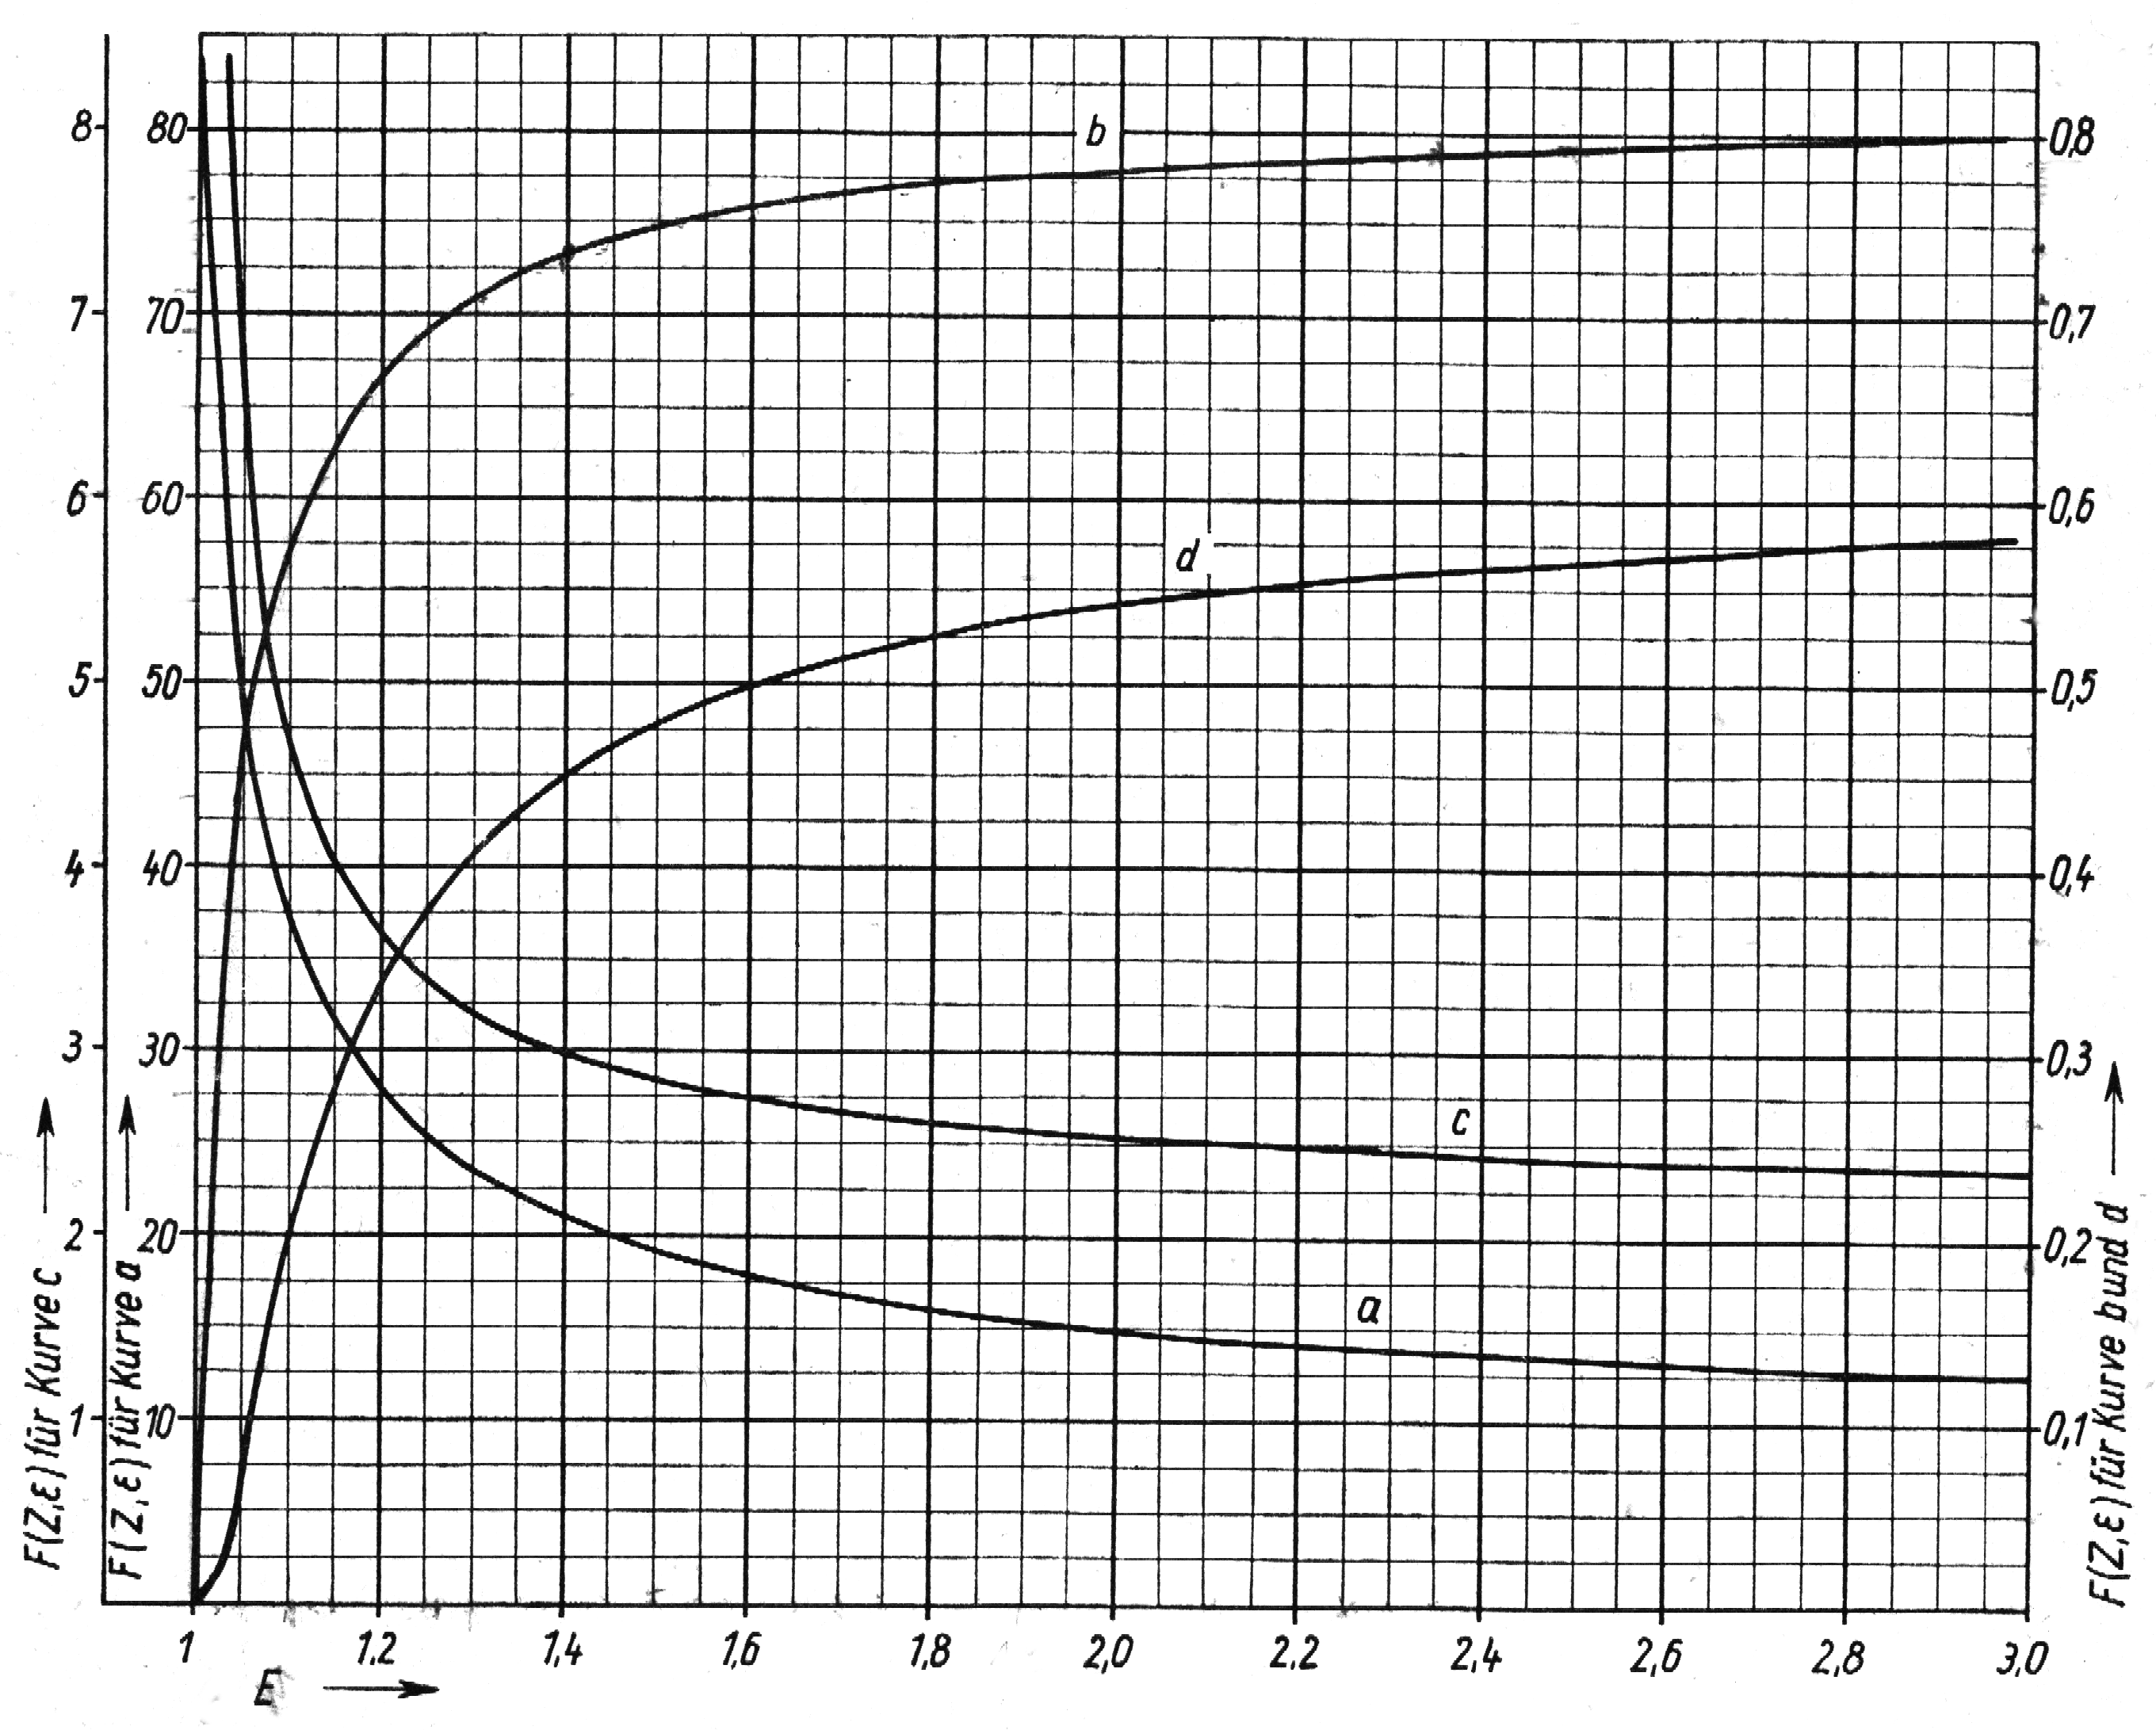
\includegraphics[width=\linewidth]{../Fermifunktion.png}
    \caption{%
        Fermi-Funktion $F(Z, \epsilon)$ für den $\betaminus$-Übergang von
        Hf$^{181}$ (Kurve a), $\betaplus$-Übergang von Na$^{22}$ (Kurve b),
        $\betaminus$- und $\betaplus$-Übergang von Cu$^{64}$ (Kurve c bzw\@.
        d). Aus \parencite[Fig. 111]{Riezler/Kernphysikalisches} mit
        freundlicher Erlaubnis des Springer-Verlags.
    }
    \label{fig:fermifunktion}
\end{figure}

\subsection{Kuriedarstellung}

In der Kuriedarstellung\footnote{Nach F.\,N.\,D\@.~Kurie, nicht Marie Curie
\parencite{wikipedia/Kurie}} trägt man nicht die Zählrate gegen die kinetische
Energie auf, sondern transformiert die Zählrate zur Größe $K$ wie folgt
\parencite[(138)]{Riezler/Kernphysikalisches}:
\[
    K(\epsilon) = \sqrt{\frac{\dot N(\epsilon)}{F(Z, \epsilon) \eta(\epsilon) \epsilon}}.
\]
Dadurch entsteht im Diagram eine Gerade, die die Abszisse bei $E_0$ schneidet,
sofern die Neutrinos masselos sind. Haben die Neutrinos eine endliche Masse, so
wird der Schnittpunkt bei etwas kleineren Energien liegen, da nicht die volle
Zerfallsenergie als kinetische Energie für das Elektron zur Verfügung steht.

\section{Spektrometeraufbau}

Die beiden für diese Art Versuche interessanten Spektrometer sind das
Halbkreisspektrometer und das doppeltfokussierende $\piup \sqrt
2$-Spektrometer.

Das Halbkreisspektrometer arbeitet mit einem Permanentmagneten, der die
Elektronen auf einer Kreisbahn arbeitet. Jedoch werden Elektronen mit gleicher
Energie nicht auf ganz genau auf einen Punkt fokussiert, sondern in einem
Bereich $\Deltaup x$ verschmiert
\parencite[§2.231]{Riezler/Kernphysikalisches}. Je größer der Sollradius
$\rho_0$ ist, desto besser wird die Abbildung nach 
\[
    \Deltaup x = s + \frac{j^2}{\piup^2 \rho} + \rho \phi^2,
\]
wobei $s$ und $h$ die Breite und Höhe der Probe und $\phi$ der halbe
Öffnungswinkel der Strahlen aus der Probe sind
\parencite[(123)]{Riezler/Kernphysikalisches}.

Eine bessere Fokussierung schafft das doppeltfokussierende $\piup \sqrt
2$-Spektrometer durch ein inhomogenes Magnetfeld. Man nutzt dazu
ein rotationssymmetrisches Magnetfeld mit einem radialen Gradienten. In
\parencite[§2.232]{Riezler/Kernphysikalisches} wird nun folgende Herleitung der
benötigten Radialabhängigkeit $B(\rho)$ sowie des benötigten
Spektrometerwinkels $\Phi$ gegeben:

Sei der Sollkreis mit Radius $\rho_0$ durch den Elektronenimpuls $p$ durch $p =
e B \rho_0$ bestimmt. Ein Teilchen, dass in einem Winkel $\phi_\rho$ zum
Sollkreis von dessen Rand startet, schneidet ihn wieder am Rand um den Winkel
$\Phi_\rho$ versetzt. Für diesen Winkel gilt für kleine $\phi_\rho$:
\parencite[(125)]{Riezler/Kernphysikalisches}
\[
    \Phi_\rho = \piup \cdot \del{1 + \frac{\rho_0}{B(\rho_0)} \dpd B
    \rho}^{-\frac 12}.
\]

In der axialen Richtung gilt eine ähnliche Bedingung:
\parencite[(126)]{Riezler/Kernphysikalisches}
\[
    \Phi_z = \piup \cdot \del{- \frac{\rho_0}{B(\rho_0)} \dpd B
    \rho}^{-\frac 12}.
\]

Aus diesen beiden Gleichungen folgt laut den Autoren nun die Beziehung:
\parencite[(127)]{Riezler/Kernphysikalisches}
\[
    \frac1{\Phi_\rho^2} + \frac1{\Phi_z^2} = \frac1{\piup^2}.
\]

Mit der Bedingung, dass diese beiden Winkel gleich sein müssen ist die Lösung
der entsprechenden Differentialgleichung:
\parencite[(129)]{Riezler/Kernphysikalisches}
\[
    \Phi = \piup \sqrt 2 \approx \SI{256}{\degree}.
\]

Daher hat dieses Spektrometer seinen Namen.

Das Spektrometer hat noch eine Dispersion, so dass die Impulsintervalle nicht
gleich groß sind. Die Dispersion ist angegeben als:
\parencite[(130)]{Riezler/Kernphysikalisches}
\[
    \gamma = \frac{4 \rho_0}{B \rho},
\]
weshalb die Messwerte mit $\gamma$ zu multiplizieren sind. Da wir die Energie
mit den Konversionslinien eichen werden, ist jede zum Impuls proportionale
Größe geeignet \parencite[§P523.5.4]{physik512-Anleitung}.

\section{Detektoren}

In diesem Versuch benötigen wir im Detektor keine Energieinformation, da wir
diese bereits durch das Magnetfeld erhalten. Wichtiger ist, dass alle
Elektronen detektiert werden und die Totzeit gering ist.

Ein möglicher Detektor ist das Geiger-Müller Zählrohr, bei dem eintretende
Teilchen ein Gas ionisieren und somit eine Hochspannungsentladung auslösen. Der
Strompuls kann verstärkt und gezählt werden.

Eine Diode, die in Sperrrichtung betrieben wird, eignet sich ebenfalls als
Detektor. Tritt ein Elektron in den die Sperrzone ein, erzeugt es dort freie
Ladungsträger (Elektronen und Löcher), die dann ebenfalls zu einem Strompuls
führen.

\section{Hysterese}

Eisen ist ferromagnetisch, es behält seine Magnetisierung $M$ auch ohne
angelegtes Magnetfeld $H$ bei. Legt man Eisen in ein Magnetfeld und erhöht die
Flussdichte bis zu einem Maximum (so dass die Magnetisierung in Sättigung geht)
und erniedrigt wieder bis $H = 0$, so nennt man die verbleibende Magnetisierung
\emph{Remanenzfeld}. Dieser Effekt ist isotrop, so dass man durch den
Mittelwert der beiden Remanenzfeldstärken die neutrale Mitte herausfinden kann.

Möchte man einen Ferromagneten entmagnetisieren, muss man das Magnetfeld, indem
sich der Ferromagnet befindet, in mehreren Durchläufen zwischen dem positiven
und negativen Maximum regeln, wobei ab dem zweiten Durchlauf der
Betrag der maximalen Magnetfeldstärke reduziert wird. Dadurch wird das
Remanenzfeld bei jedem Durchlauf schwächer, bis am Ende verschwindet. Diesen
Vorgang nennt man \emph{Hysterese}. Dieser Vorgang ist in
Abbildung~\ref{fig:hysterese} dargestellt.

\begin{figure}[htbp]
    \centering
    \begin{tikzpicture}
        \begin{axis}[
                width=\linewidth,
                height=0.7\linewidth,
                xlabel=Spulenstrom / wilk.\,Einh.,
                ylabel=Flussdichte / wilk.\,Einh.,
            ]
            \addplot[black] table [x index=1, y index=2]{../Daten/data.txt};
        \end{axis}
    \end{tikzpicture}
    \caption{%
        Hysteresekurve von Eisen. Messdaten aus \parencite{Ueding/248}.
    }
    \label{fig:hysterese}
\end{figure}

\chapter{Durchführung}

\section{Offsetspannung}

Wir erhöhen den Magnetstrom bis die Magnetisierung in Sättigung geht. Die
Hallsonde zeigt \num{-183.2(2)}\footnote{\erklaerungFehlerNotation} an. Wir
notieren die Remanenz. Nach dem Umpolen erreichen wir eine Sättigung von
\num{196}.

% TODO Tabelle mit Remanenzwerten.

\section{Kalibrierung des $\betaup$-Spektrometers}

Wir setzen die Caesiumprobe ein und evakuieren das Spektrometer wieder. Bei
\SI{4}{\percent} Transmission.

\begin{figure}[htpb]
    \centering
    \begin{tikzpicture}
        \begin{axis}[
                ybar,
                width=.7\linewidth,
                height=.4\linewidth,
                xlabel=Hallspannung/Skt.,
                ylabel=Ereignisse,
                axis lines=left
            ]
            \addplot[draw=black] table {../Daten/01-Cs-40s.txt};
        \end{axis}
    \end{tikzpicture}
    \caption{%
        $\betaup$-Spektrum von ${}^{137}$Cs bei \SI{40}{\second}
        Messdauer und \SI{4}{\percent} Transmission
    }
    \label{fig:Cs-40s-vollst}
\end{figure}

\begin{figure}[htpb]
    \centering
    \begin{tikzpicture}
        \begin{axis}[
                width=.7\linewidth,
                height=.4\linewidth,
                xlabel=Hallspannung/Skt.,
                ylabel=Ereignisse,
                axis lines= left
            ]
            \addplot[black] table {../Daten/02-Cs-40s.txt};
        \end{axis}
    \end{tikzpicture}
    \caption{%
        $\betaup$-Spektrum von ${}^{137}$Cs bei \SI{40}{\second}
        Messdauer und \SI{4}{\percent} Transmission
    }
    \label{fig:Cs-40s-ausschn}
\end{figure}

\begin{figure}[htpb]
    \centering
    %\begin{tikzpicture}
    %    \begin{axis}[width=.7\linewidth, height=.4\linewidth,
    %        xlabel=Hallspannung/Skt., ylabel=Ereignisse, axis lines= left]
    %        \addplot[black] table {../Daten/01-Cs-100s.txt};
    %    \end{axis}
    %\end{tikzpicture}
    \caption{%
        $\betaup$-Spektrum von ${}^{137}$Cs bei \SI{100}{\second}
        Messdauer und \SI{1}{\percent} Transmission
    }
    \label{fig:Cs-100}
\end{figure}

\chapter{Auswertung}

\IfFileExists{\bibliographyfile}{
    \printbibliography
}{}

\end{document}

% vim: spell spelllang=de tw=79
